\begin{problem}[Chebyshev polynomials and their properties]\label{prob:ChebPolyProp}
  
  Let $T_{n}\in\Pol{n}$ be the $n$-th Chebyshev polynomial, as defined in \lref{def:Tpol} and $\xi_0^{(n)},\dots,\xi_{n-1}^{(n)}$ be the $n$ zeros of $T_n$. According to  \lref{eq:TPN}, these are given by
\begin{equation}\label{eq:zeros}
  \xi^{(n)}_{j} = \cos\left(\frac{2j+1}{2n}\,\pi\right)\;\bcom
    \quad j=0,\ldots,n-1.
\end{equation}
  We define the family of discrete $L^2$ semi inner products, \emph{cf.} \lref{eq:dSPLtwo},
\begin{equation}\label{eq:discrete}
  (f,g)_n:=\sum_{j=0}^{n-1} f(\xi_j^{(n)}) g(\xi_j^{(n)}),\quad f,g\in C^0([-1,1])
\end{equation}
and the special weighted $L^2$ inner product
\begin{equation}\label{eq:weighted}
  (f,g)_w:=\int_{-1}^1 \frac{1}{\sqrt{1-t^2}} f(t) g(t)\,dt \quad f,g\in C^0([-1,1])
\end{equation}

% SUBPROBLEM 1
\begin{subproblem}[2] 
    Show that the Chebyshev polynomials are an orthogonal family of polynomials with respect to the inner product defined in \eqref{eq:weighted} according to \lref{def:onp}, namely $(T_k,T_l)_w=0$ for every $k\neq l$.

    \begin{hint}
      Recall the trigonometric identity $2\cos(x)\cos(y) = \cos(x+y)+\cos(x-y)$.
    \end{hint}

\begin{solution}
For $k,l=0,\dots,n$ with $k\neq l$, by using the substitution $s=\arccos t$ ($ds=- \frac{1}{\sqrt{1-t^2}}\,dt$) and simple trigonometric identities we readily compute
\[
\begin{split}
(T_k,T_l)_w &= \int_{-1}^1 \frac{1}{\sqrt{1-t^2}} \cos(k\,\arccos t) \cos(l\,\arccos t)\,dt \\
&= \int_{0}^\pi  \cos(k s) \cos(l s)\,ds \\
&=\frac{1}{2} \int_{0}^\pi  \cos((k+l) s) + \cos((k-l) s)\,ds \\
&= \frac{1}{2}( [\sin((k+l)s)/(k+l)]^\pi_0 + [\sin((k-l)s)/(k-l)]^\pi_0)\\
&=0,
\end{split}
\]
since $k+l\neq 0$ and $k-l\neq 0$.
\end{solution}
\end{subproblem}

Consider the following statement.

\fbox{\parbox{0.95\textwidth}{
\textbf{Theorem}. The family of polynomials $\{T_0,\dots,T_n\}$ is an orthogonal
basis ($\to$ \lref{def:onb}) 
of $\Pol{n}$ with respect to the inner product $(\; ,\,)_{n+1}$ defined in \eqref{eq:discrete}.
}}

% SUBPROBLEM 2
\begin{subproblem}[2] 
Write a C++ code to test the assertion of the theorem.

\begin{hint}
  \lref{chebpolmult} demonstrates the efficient evaluation of Chebychev
  polynomials based on their 3-term recurrence formula from \lref{rem:3termCheb}.
\end{hint}

   \begin{solution}
As a consequence of \lref{rem:3termCheb}, we already know that $\{T_0,\dots,T_n\}$
is a basis for $\Pol{n}$. We check the orthogonality in the C++ code given in
Listing~\ref{ChebOrthog}.
\lstinputlisting[caption={Orthogonality of Chebyshev polynomials},label={ChebOrthog}]
 {\problems/ch_polynomialinterpolation/CPP/ChebOrthog.cpp}
\end{solution}
\end{subproblem}

% SUBPROBLEM 3
\begin{subproblem}[4] 
Prove the theorem.

\begin{hint}
  Use the relationship of trigonometric functions and the complex exponential
  together with the summation formula for geometric sums. 
\end{hint}

   \begin{solution}
It remains to check the orthogonality condition, namely that $(T_k,T_l)_n=0$ for $k\neq l$. For $k,l=0,\dots,n+1$ with $k\neq l$  by \eqref{eq:zeros}  we have
\begin{equation}\label{eq:norm}
\begin{split}
(T_k,T_l)_{n+1} &= \sum_{j=0}^{n} T_k(\xi_j^{(n)}) T_l(\xi_j^{(n)}) \\
&= \sum_{j=0}^{n} \cos\left(k \frac{2j+1}{2(n+1)}\,\pi\right) \cos\left(l \frac{2j+1}{2(n+1)}\,\pi\right) \\
&=\frac{1}{2} \sum_{j=0}^{n}( \cos\left((k+l) \frac{2j+1}{2(n+1)}\,\pi\right) + \cos\left((k-l) \frac{2j+1}{2(n+1)}\,\pi\right) ).\\
\end{split}
\end{equation}
It is now enough to show that 
\begin{equation}\label{eq:geometric}
\sum_{j=0}^{n} \cos\left(m \frac{2j+1}{2(n+1)}\,\pi\right)=0,\qquad m\in\Z^*.
\end{equation}
In order to verify this, observe that
\[
\sum_{j=0}^{n} \cos \left( m \frac{2j+1}{2(n+1)}\,\pi \right)= 
\Re ( \sum_{j=0}^{n} e^{i m \frac{2j+1}{2(n+1)}\,\pi}  )
= \Re ( e^{i m \frac{1}{2(n+1)}\,\pi} \sum_{j=0}^{n} e^{i m \frac{j}{n+1}\,\pi}  ).
\]
Finally, by the standard formula for the geometric sum we have
\begin{align*}
e^{i m \frac{1}{2(n+1)}\,\pi} \sum_{j=0}^{n} e^{i m \frac{j}{n+1}\,\pi } =e^{i m \frac{1}{2(n+1)}\,\pi}\frac{1-e^{i m \frac{n+1}{n+1}\,\pi} }{1-e^{i m \frac{1}{n+1}\,\pi}} \\
=\frac{1-e^{i m \pi} }{e^{-i m \frac{1}{2(n+1)}\,\pi}-e^{i m \frac{1}{2(n+1)}\,\pi}} = - \frac{1-e^{i m \pi}}{2} \frac{1}{i \sin{m \frac{1}{2(n+1)}\,\pi}} \in i \IR,
\end{align*}
implying $\Re ( e^{i m \frac{1}{2(n+1)}\,\pi} \sum_{j=0}^{n} e^{i m \frac{j}{n+1}\,\pi}  ) = 0$ as desired.
\end{solution}
\end{subproblem}

% SUBPROBLEM 4
\begin{subproblem}[2] 
  Given a function $f\in C^0([-1,1]$, find an expression for the best approximant
  $q_n\in\Pol{n}$ of $f$ in the discrete $L^{2}$-norm:
\[
q_n=\argmin_{p\in\Pol{n}} \norm{f-p}_{n+1},
\]
where $\norm{\;}_{n+1}$ is the norm induced by the scalar product
$(\;,\,)_{n+1}$. You should express $q_n$ through an expansion in Chebychev
polynomials of the form
\begin{equation}\label{eq:alpha}
q_n=\sum_{j=0}^n \alpha_j T_j
\end{equation}
for suitable coefficients $\alpha_j\in\R$.
\begin{hint}
The task boils down to determining the coefficients $\alpha_{j}$. 
Use the theorem you have just proven and a slight extension of \lref{cor:msba:onb}.
\end{hint}
\begin{solution}
In view of the theorem, the family $\{T_0,\dots,T_n\}$ is an orthogonal basis of $\Pol{n}$ with respect to the inner product $(\; ,\,)_{n+1}$. By \eqref{eq:norm} and \eqref{eq:geometric} we have
\begin{equation}\label{eq:lambda}
\lambda_k^2:=\norm{T_k}^2_{n+1}=(T_k,T_k)_{n+1}=
\begin{cases}
\frac{1}{2}\sum_{j=0}^n(\cos(0) + \cos(0))=n+1 & \text{if $k=0$},\\
\frac{1}{2}\sum_{j=0}^n \cos(0)=(n+1)/2 & \text{otherwise.}
\end{cases}
\end{equation}
The family $\{T_k/\lambda_k:k=0,\dots,n\}$ is an ONB of $\Pol{n}$ with respect to the inner product $(\; ,\,)_{n+1}$. Hence, by \lref{cor:msba:onb} we have that
\[
q_n=\sum_{j=0}^n\, (f,T_j/\lambda_j)_{n+1}\, \frac{T_j}{\lambda_j}=\sum_{j=0}^n \alpha_j T_j,\quad \alpha_j=\frac{1}{n+1}
\begin{cases}
{(f,T_j)_{n+1}} & \text{if $k=0$},\\
2 {(f,T_j)_{n+1}}& \text{otherwise.}
\end{cases}
\]
\end{solution}
\end{subproblem}

% SUBPROBLEM 5
\begin{subproblem}[2]
Write a C++ function
\begin{lstlisting}
template <typename Function>
void bestpolchebnodes(const Function &f, Eigen::VectorXd &alpha)
\end{lstlisting}
that returns the vector of coefficients $(\alpha_j)_j$ in \eqref{eq:alpha} given a function $f$. Note that the degree of the polynomial is indirectly passed with the length of the output \texttt{alpha}. The input \texttt{f} is a lambda-function, e.g.
\begin{lstlisting}
auto f = [] (double & x) {return 1/(pow(5*x,2)+1);};
\end{lstlisting}


\begin{solution}
See file \texttt{ChebBest.cpp}.
\end{solution}
\end{subproblem}

% SUBPROBLEM 6
\begin{subproblem}[2] 
Test \texttt{bestpolchebnodes} with the function $f(x)=\frac{1}{(5x)^2+1}$ and
$n=20$. Approximate the supremum norm of the approximation error by sampling on an
equidistant grid with $10^{6}$ points. 

\begin{hint}
  Again, \lref{chebpolmult} is useful for evaluating Chebychev polynomials. 
\end{hint}


% Copy and paste the vector of coefficients obtained to Matlab and plot the result, comparing it with $f$. Use the Matlab built-in function \texttt{chebyshevT}.
   \begin{solution}
See file \texttt{ChebBest.cpp}. The output (plotted with Matlab) is shown in Figure~\ref{fig:ChebBest}.
\begin{figure}\begin{center}
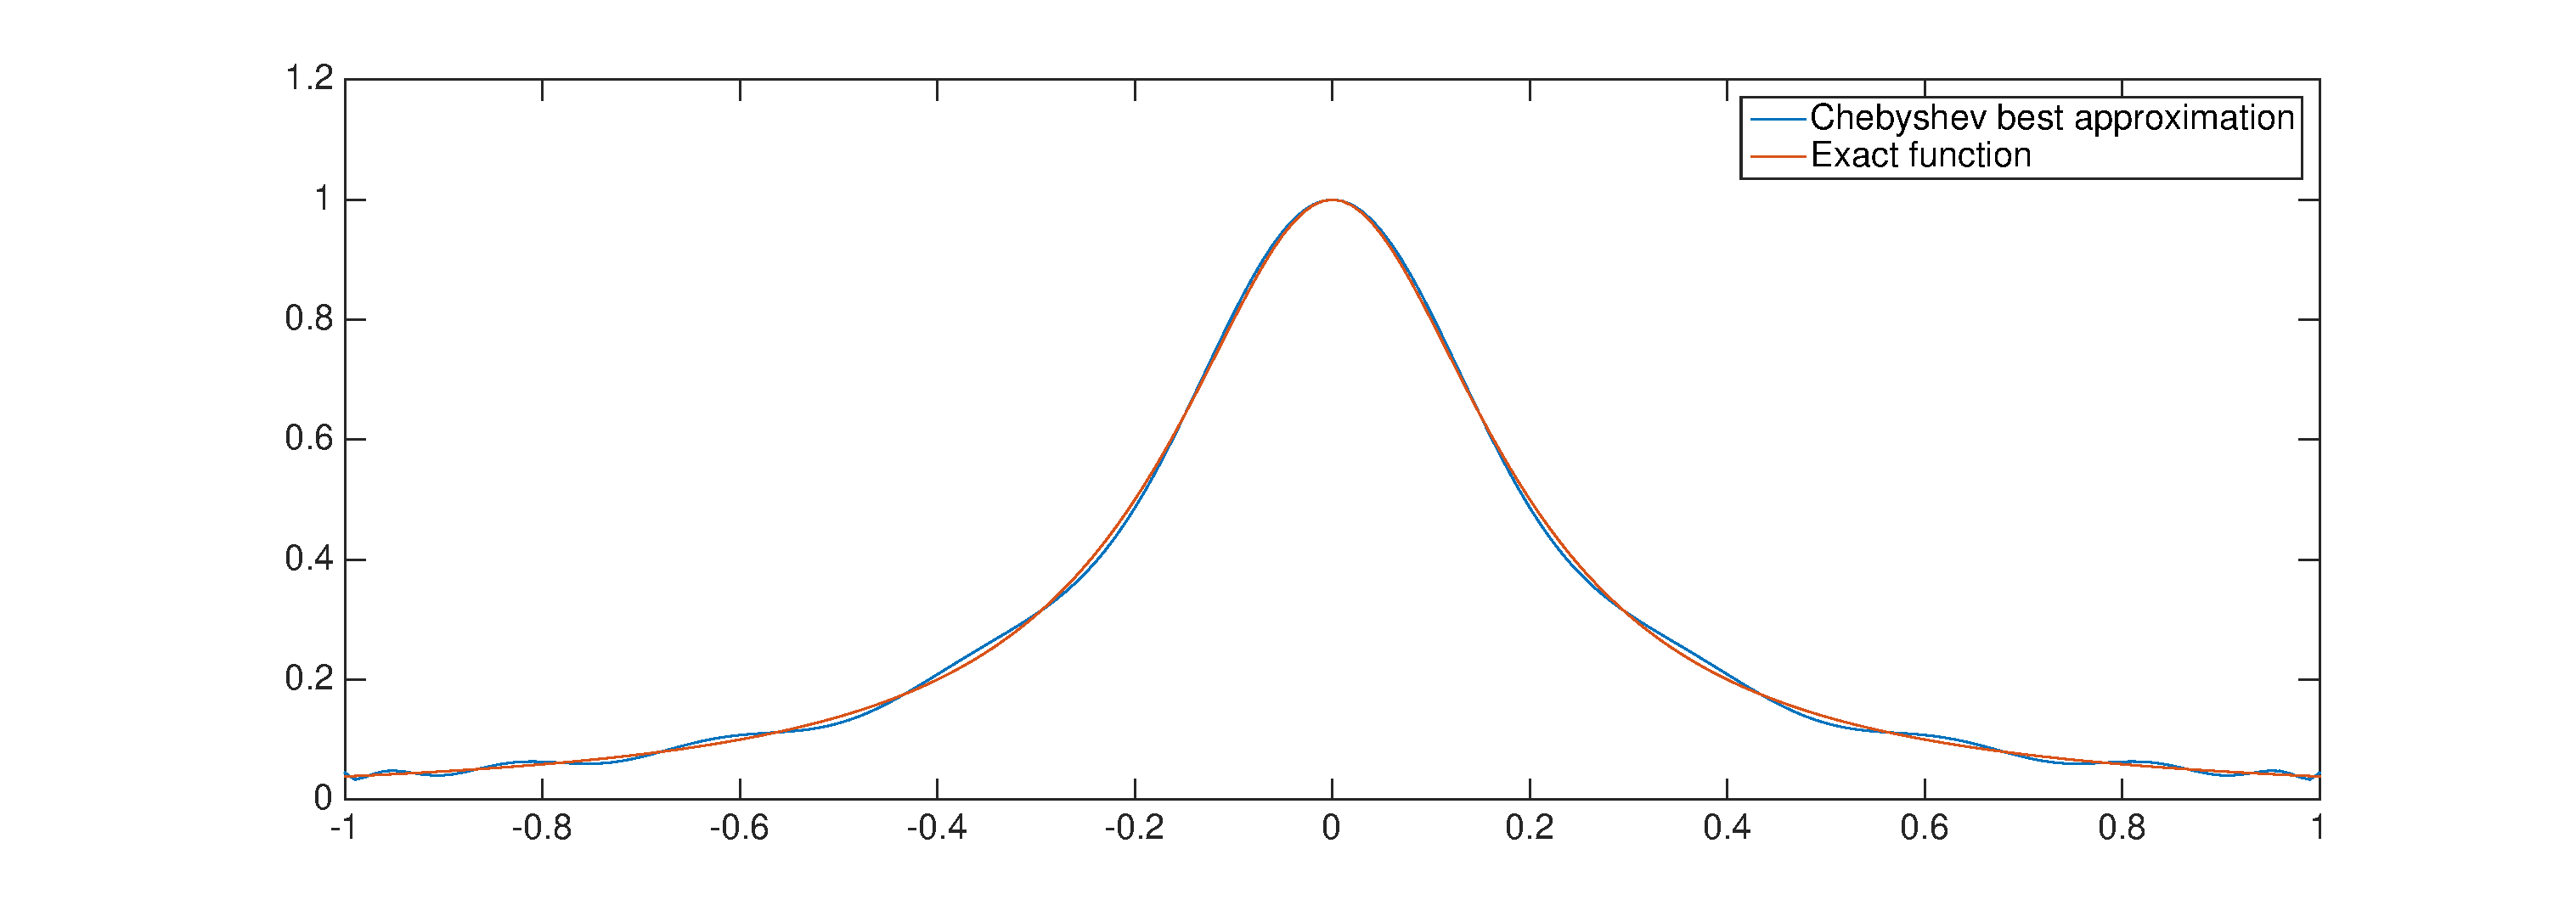
\includegraphics[width = \textwidth]{\problems/ch_polynomialinterpolation/PICTURES/ChebBest.eps}
\caption{The result of code \texttt{ChebBest.m}.}
\label{fig:ChebBest}
\end{center}\end{figure}
\end{solution}
\end{subproblem}

% SUBPROBLEM 7
\begin{subproblem}[2] 
Let $L_j$, $j=0,\dots,n$, be the Lagrange polynomials associated with the nodes
$t_j=\xi^{(n+1)}_{j}$ of Chebyshev interpolation with $n+1$ nodes on $[-1,1]$, see
\lref{eq:TPN}. Show that
\[
L_j = \frac{1}{n+1} + \frac{2}{n+1} \sum_{l=1}^n T_l(\xi^{(n+1)}_{j}) T_l.
\]

\begin{hint}
  Again use the above theorem to express the coefficients of a Chebychev expansion
  of  $L_{j}$. 
\end{hint}

   \begin{solution}
We have already seen that $\{T_l/\lambda_l:l=0,\dots,n\}$ is an ONB of $\Pol{n}$. Thus we can write
\[
L_j=\sum_{l=0}^n \frac{(L_j,T_l)_{n+1}}{\lambda_l^2} T_l =\sum_{l=0}^n \sum_{k=0}^n L_j(\xi^{(n+1)}_{k}) T_l(\xi^{(n+1)}_{k}) \frac{T_l}{\lambda_l^2} 
\]
By definition of Lagrange polynomials we have $ L_j(\xi^{(n+1)}_{k}) = \delta_{jk}$, whence
\[
L_j=\sum_{l=0}^n  T_l(\xi^{(n+1)}_{l}) \frac{T_l}{\lambda_l^2}.
\]
Finally, the conclusion immediately follows from \eqref{eq:lambda}.
\end{solution}
\end{subproblem}

\end{problem}




